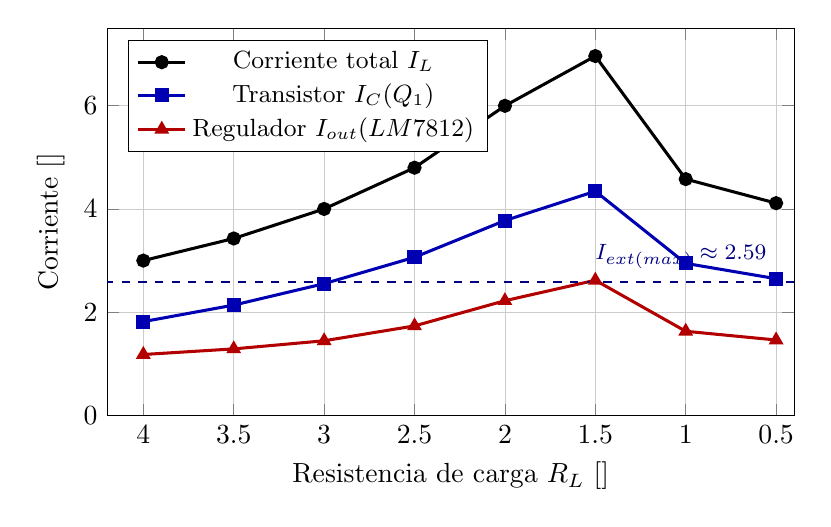
\begin{tikzpicture}
\begin{axis}[
    width=0.85\textwidth,
    height=6.5cm,
    xlabel={Resistencia de carga $R_L$ [\si{\ohm}]},
    ylabel={Corriente [\si{\ampere}]},
    grid=both,
    grid style={line width=.1pt, draw=gray!20},
    major grid style={line width=.2pt, draw=gray!40},
    x dir=reverse,
    xmin=0.4, xmax=4.2,
    ymin=0, ymax=7.5,
    legend pos=north west,
    legend style={font=\small}
]

% Corriente total de carga
\addplot[
    color=black,
    mark=*,
    mark size=2pt,
    line width=1.1pt
] coordinates {
    (4.0, 3.000)
    (3.5, 3.428)
    (3.0, 4.000)
    (2.5, 4.799)
    (2.0, 5.997)
    (1.5, 6.961)
    (1.0, 4.578)
    (0.5, 4.112)
};
\addlegendentry{Corriente total $I_L$}

% Corriente de colector de Q1
\addplot[
    color=blue!70!black,
    mark=square*,
    mark size=2pt,
    line width=1.1pt
] coordinates {
    (4.0, 1.818)
    (3.5, 2.138)
    (3.0, 2.553)
    (2.5, 3.064)
    (2.0, 3.775)
    (1.5, 4.343)
    (1.0, 2.946)
    (0.5, 2.649)
};
\addlegendentry{Transistor $I_C(Q_1)$}

% Corriente de salida del LM7812
\addplot[
    color=red!70!black,
    mark=triangle*,
    mark size=2pt,
    line width=1.1pt
] coordinates {
    (4.0, 1.181)
    (3.5, 1.290)
    (3.0, 1.447)
    (2.5, 1.735)
    (2.0, 2.223)
    (1.5, 2.619)
    (1.0, 1.631)
    (0.5, 1.462)
};
\addlegendentry{Regulador $I_{out}(\text{LM7812})$}

% Limite teorico de Ic1max
\addplot[dashed, color=blue!50!black, line width=0.8pt] coordinates {
    (0.4, 2.59) (4.2, 2.59)
};
\node[anchor=south east, text=blue!50!black, font=\footnotesize] at (axis cs: 0.5, 2.65) {$I_{ext(max)} \approx \SI{2.59}{\ampere}$};

\end{axis}
\end{tikzpicture}
